\Block{Introduction}{

\textbf{Geoid Problem}
\begin{itemize}
     \item (TODO)       
\end{itemize}

\textbf{Mantle Convection Problem}

\begin{figure}[H]
    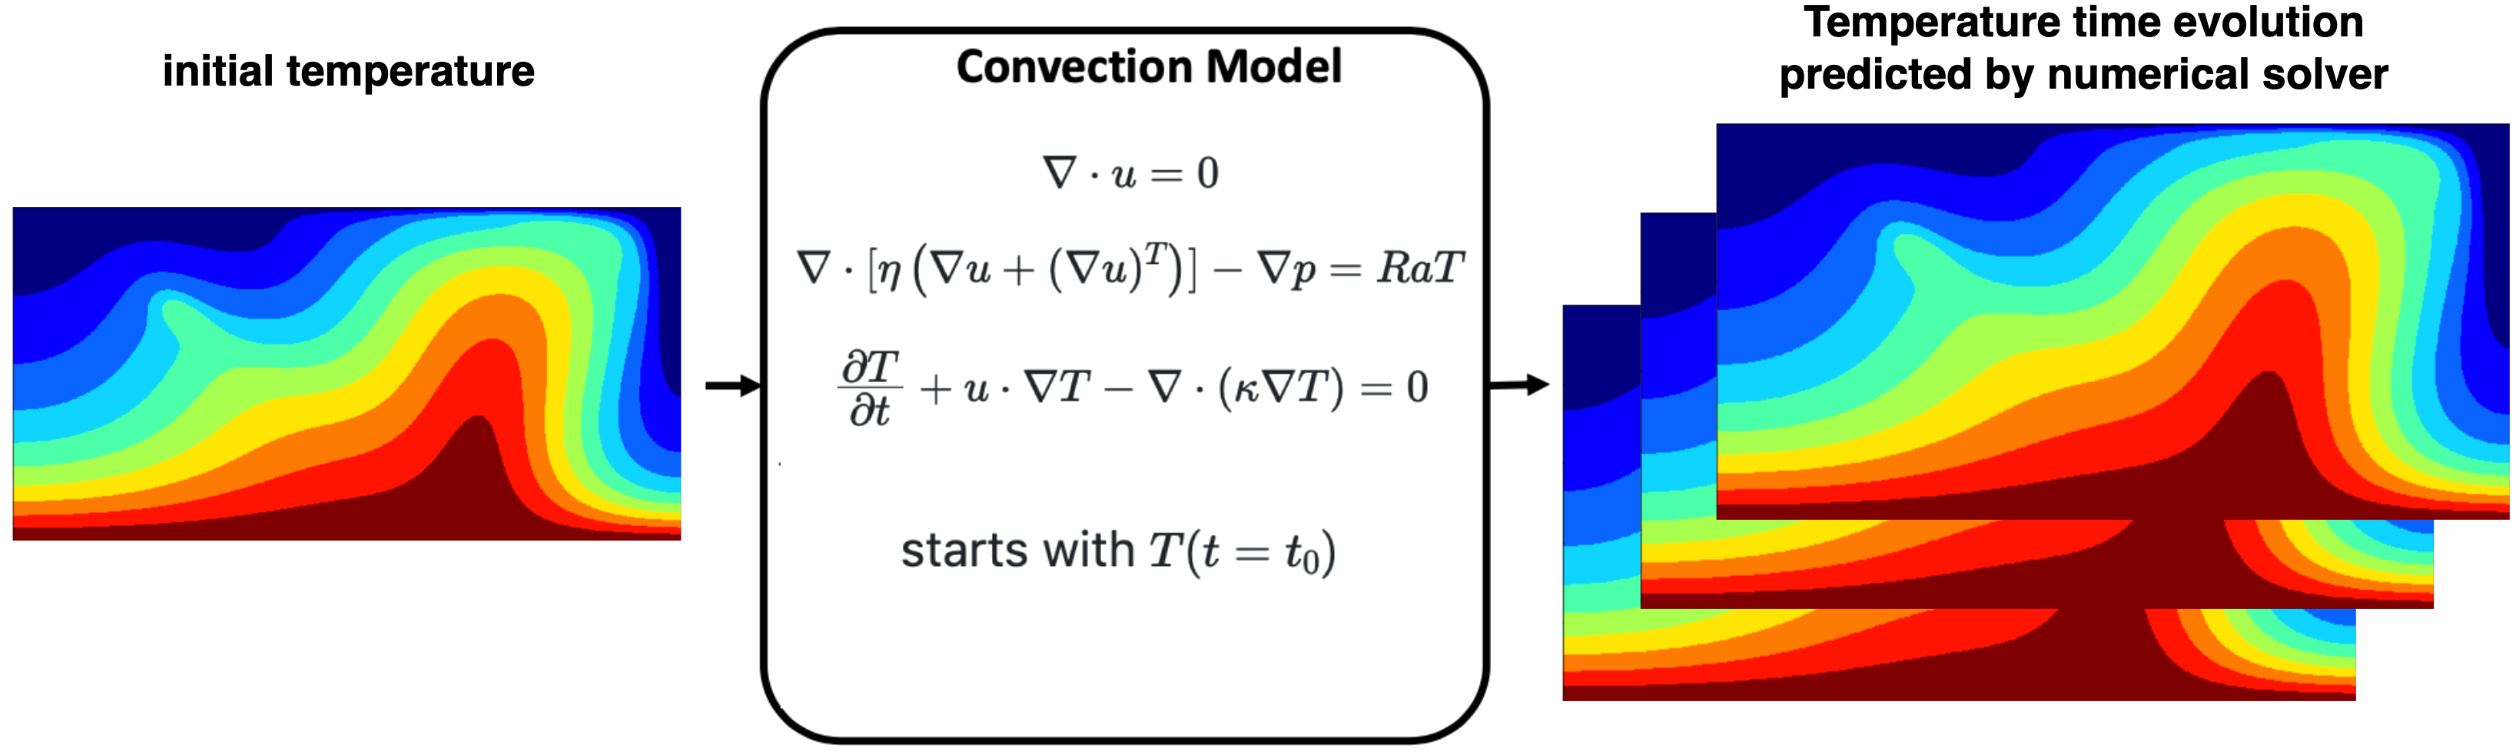
\includegraphics[width=\linewidth]{figures/Mantle_Convection_workflow.png}
    \caption{Typical Mantle Convection Workflow}
\end{figure}

\textbf{Neural Networks}
\begin{itemize}
    \item Fully Connected Neural Network (FNN)
        \begin{itemize}
            \item\begin{equation}
            \mathcal{N}(\theta) = \Theta_\text{n} \circ g \circ \Theta_\text{n-1} ... \circ g \circ \Theta_1
            \end{equation}

            \item Where \begin{equation} \Theta(x) = xA^{T} + b \end{equation}

            \item Here, FNN $\mathcal{N}$ is represented as the composition of $n$ affine maps ($n$ hidden layers) $\Theta$ and activation function $g$, where $\theta$ represents all the learnable parameters -- $A$ and $b$ in different $\Theta$. $A$ is the weight matrix (with a size of $num_\text{output neurons} \times num_\text{input neurons}$) and $b$ (with a size of $1 \times num_\text{output neurons}$) is the bias vector.
            
        \end{itemize}
    \item Convolutional Autoencoders (ConvAE)
        \begin{itemize}
            \item An encoder using convolution operation to reduce the size of the original input field and output a latent space representation

            \item A decoder using deconvolution operation to transform the latent space representation back to the original size field
        \end{itemize}
    \item Long short-term memory (LSTM)
        \begin{itemize}
            \item Use a sequence of input recurrently to predict a sequence of output.
            
            \item Handle time-series data more accurately than other networks
        \end{itemize}
        
\end{itemize}

}


\Block{Research Aims}{
(TODO)
}


\Block{Methods}{

\textbf{Geoid Problem}.
\begin{itemize}
    \item Testing on a dataset with 1000 pairs of input and output
    
        \begin{itemize}
            \item Input: a vector with 257 values
	    \item Output: a vector with 60 values      representing a set of spherical harmonic coefficients describing the geoid height on the
        surface of the Earth
        \end{itemize}  
\end{itemize}

\begin{figure}[H]
    \centering
    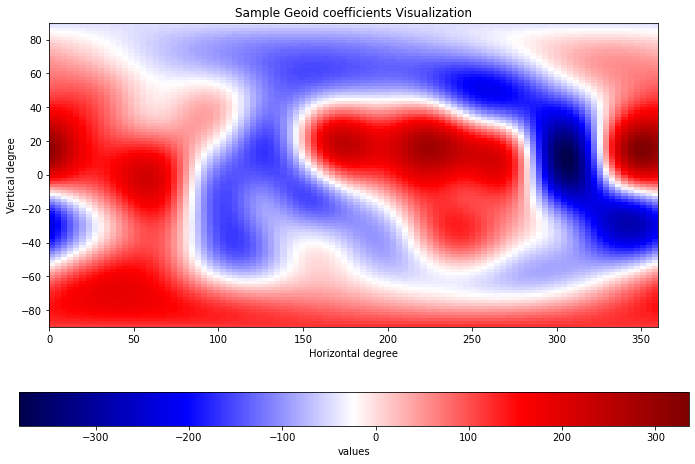
\includegraphics[width=0.5\linewidth]{figures/Geoid_Sample_visualization.png}
    \caption{Sample Geoid coefficients}
\end{figure}

\begin{itemize}
    \item Using Fully Connected Neural Networks (FNN) for prediction

    \item Systematically training and testing different FNN architectures
\end{itemize}

\bigbreak

\textbf{Mantle Convection Problem}
\begin{itemize}
    
    \item Supported by Gadi - a HPC system
    \item Testing on 3 different datasets, where each dataset is composed of various simulations that each has 100 temperature fields and 100 timestamps.
    
        \begin{itemize}
            
            \item Limited dataset: 100 simulations, varying distance between consecutive time steps
            
	    \item Larger dataset: 903 simulations,           varying distance between consecutive time steps
     
            \item Interpolated dataset: generated from the Larger dataset, 903 simulations, equal distance between consecutive time steps
        \end{itemize}
\end{itemize}

\begin{figure}[H]
    \centering
    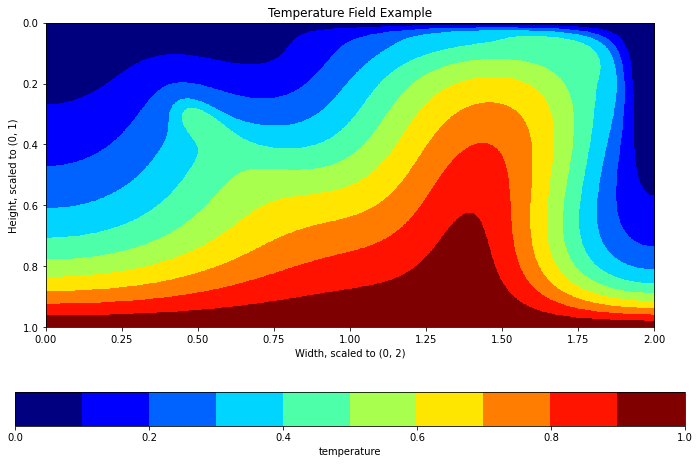
\includegraphics[width=0.5\linewidth]{figures/temperature_field_example.png}
    \caption{Sample Temperature field}
\end{figure}   

\begin{itemize}   
    
    \item Using Convolutional Autoencoders (ConvAE) to compress the data into its latent space representation.
\end{itemize}

\begin{figure}[H]
    \centering
    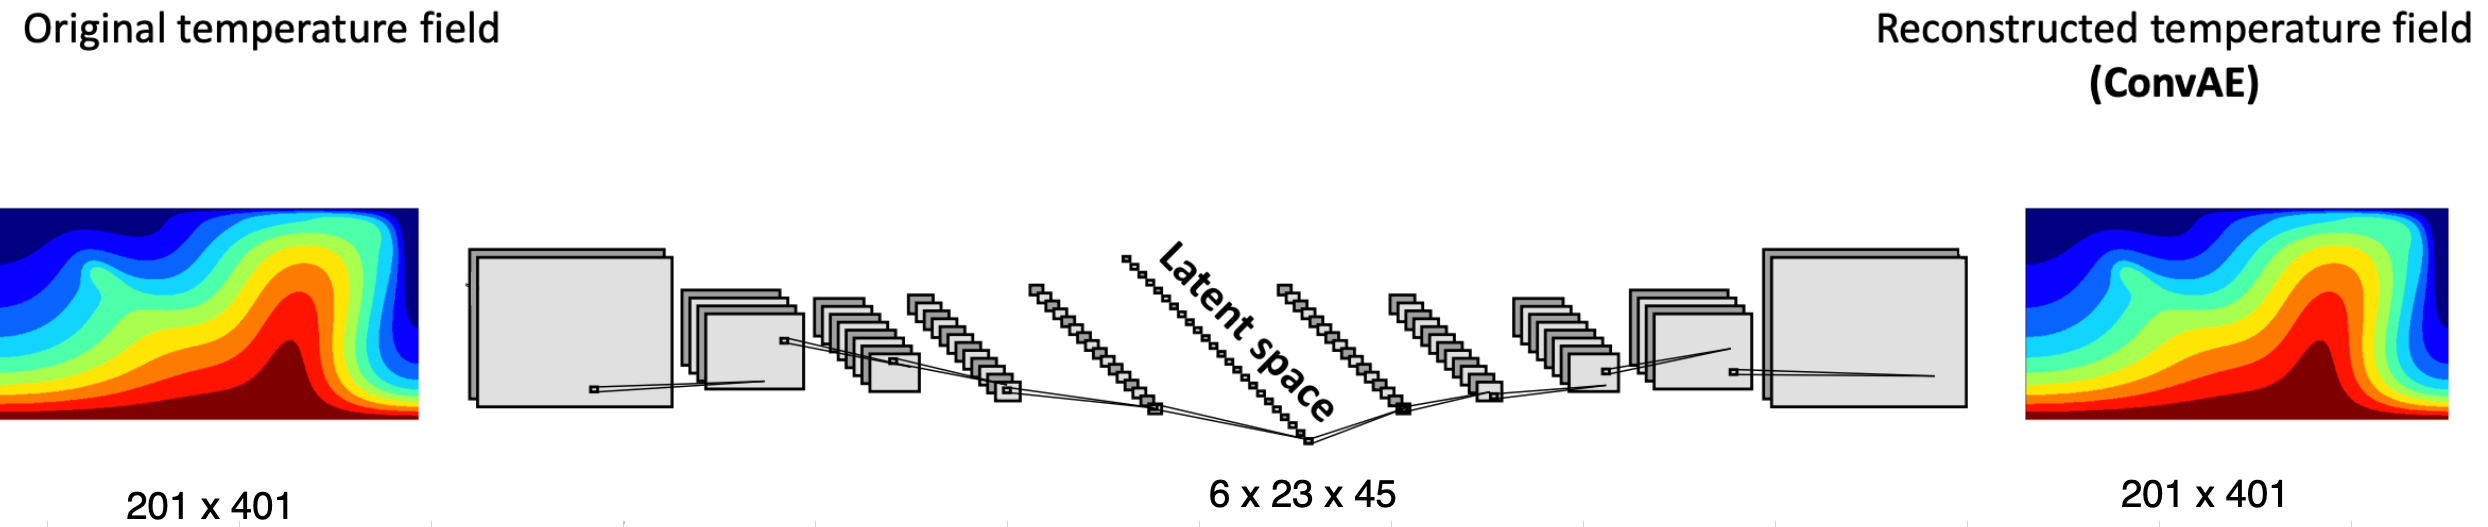
\includegraphics[width=0.8\linewidth]{figures/ConvAE_workflow.png}
    \caption{ConvAE workflow}
\end{figure}

\begin{itemize}  
    \item Given a temperature field in its latent space representation, using Fully Connected Neural Network (FNN) to predict temperature field at the next timestamp. 
\end{itemize}

\begin{figure}[H]
    \centering
    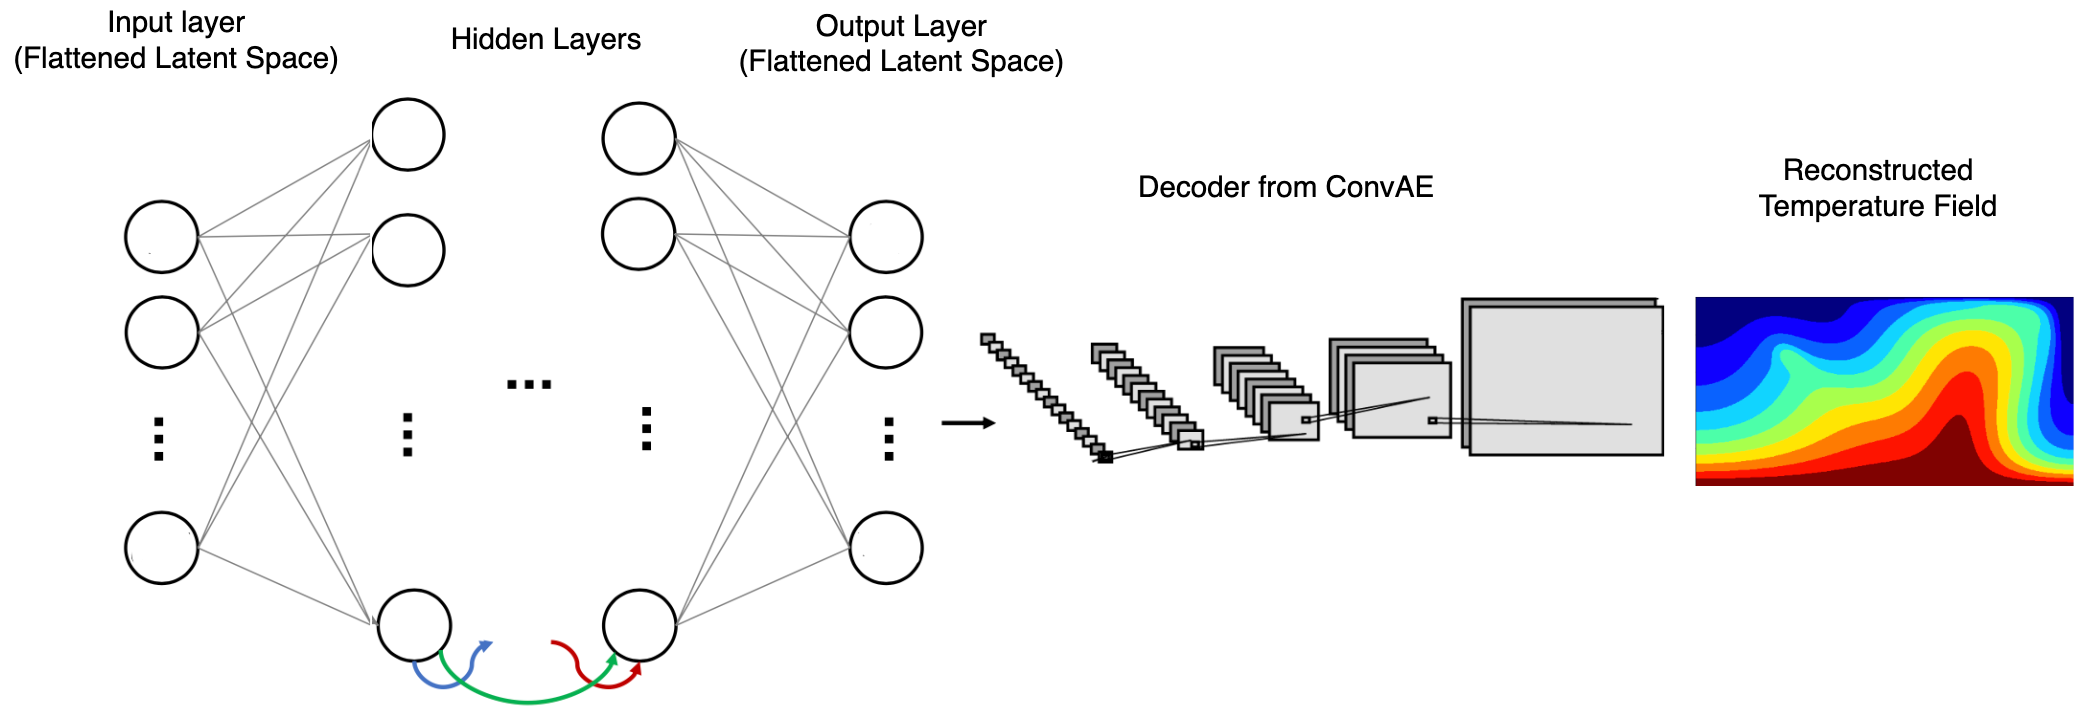
\includegraphics[width=0.8\linewidth]{figures/FNN_workflow.png}
    \caption{FNN workflow}
\end{figure}

\begin{itemize} 
    \item Two ways to predict a complete simulation using FNN:

        \begin{itemize}
            \item use $T1$ from data set $\rightarrow$ get predicted $T2$ $\rightarrow$ use predicted $T2$ $\rightarrow$ get predicted $T3$ $\rightarrow$ ...
            
            \item use $T1$ from data set $\rightarrow$ get predicted $T2$ $\rightarrow$ use $T2$ from data set $\rightarrow$ get predicted $T3$ $\rightarrow$ ...
        \end{itemize}

    \item Given the first 50 temperature fields from a simulation in its latent space representation, using Long Short-Term Memory (LSTM) to predict the last 50 temperature fields as a sequence.
     
\end{itemize}

\begin{figure}[H]
    \centering
    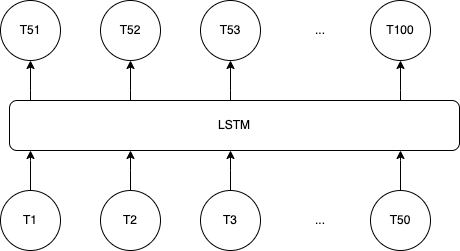
\includegraphics[width=0.8\linewidth]{figures/LSTM_workflow.png}
    \caption{General LSTM structure and the workflow in this research, reference: https://stackoverflow.com/questions/48302810/whats-the-difference-between-hidden-and-output-in-pytorch-lstm}
\end{figure}
}


\Block{Results and Findings}{

\textbf{Geoid Problem}.

\begin{itemize}
    \item FNN architectures with a total number of 4 hidden layers have the best performance when the output data is normalised using a scaler before training and testing.
\end{itemize}

\begin{figure}[H]
    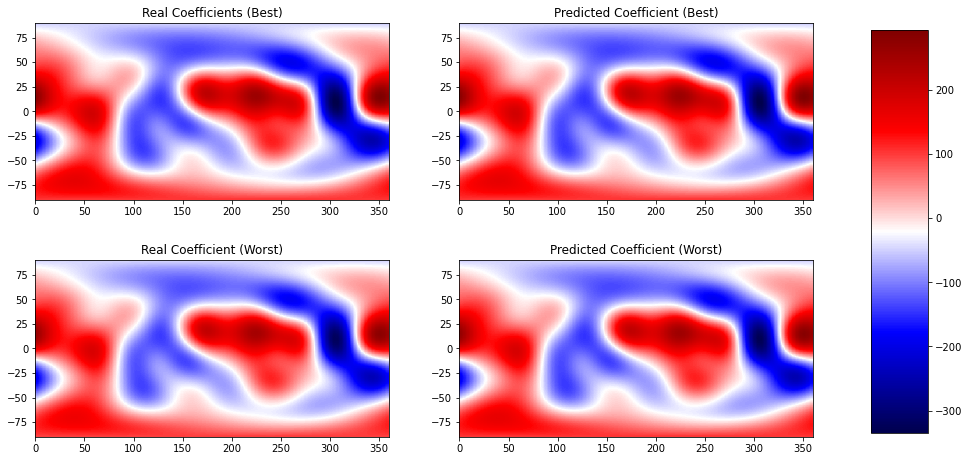
\includegraphics[width=\linewidth]{figures/Geoid_Best_Worst.png}
    \caption{Visualization of the most and the least accurate Geoid prediction}
\end{figure}

\begin{figure}[H]
    \centering
    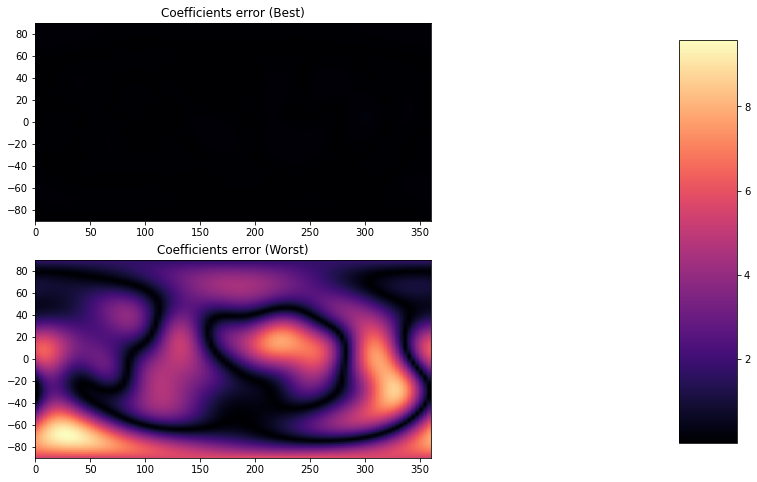
\includegraphics[width=0.5\linewidth]{figures/Geoid_Errors.png}
    \caption{Visualization of errors in the most and the least accurate Geoid prediction}
\end{figure}


\textbf{Mantle Convection Problem}

\begin{itemize}
    
    \item Limited Dataset
        \begin{itemize}
            \item ConvAE has low reconstruction error given a latent space size of 5x23x45, which offers an excellent compression factor of 13.
            
            \item FNN has low loss value when predicting the next temperature field given a total of 3 hidden layers. However, when predicting a complete simulation using FNN:
            
            \begin{itemize}
                \item output-as-input prediction fails to capture the trend of simulation in its worst case and the prediction result is completely different to the actual simulations
            
                \item while the second method mostly matches with the actual output even in its worst case.
            
            \end{itemize}

            \item LSTM has a higher loss value than FNN, but is able to capture the characteristic of the simulation more precisely

            \item predicted animations generated by FNN and LSTM are either moving faster or slower than the actual simulations
            
        \end{itemize}
        
    \item Larger Dataset
        \begin{itemize}
            \item Low reconstruction error for ConvAE given the same architecture.

            \item No significant improvement for the prediction result of FNN and LSTM.

            \item Confirmed that the lower accuracy of LSTM is not caused by some potential underfitting problem brought by the limited size of the data
            
            \item The problem of the predicted animations having inconsistent speed still exists.
            
        \end{itemize}

        
    \item Interpolated Dataset
    
    \begin{itemize}
            \item Lower reconstruction error is 3 times lower for ConvAE given the same architecture.

            \item Better performance for both FNN and LSTM.
            
            \item The problem of the predicted animations having inconsistent speed with the actual one is now solved. Confirmed that this problem is caused by the varying distance between consecutive time steps
            
    \end{itemize} 
 
        
\end{itemize}

\begin{figure}[H]
    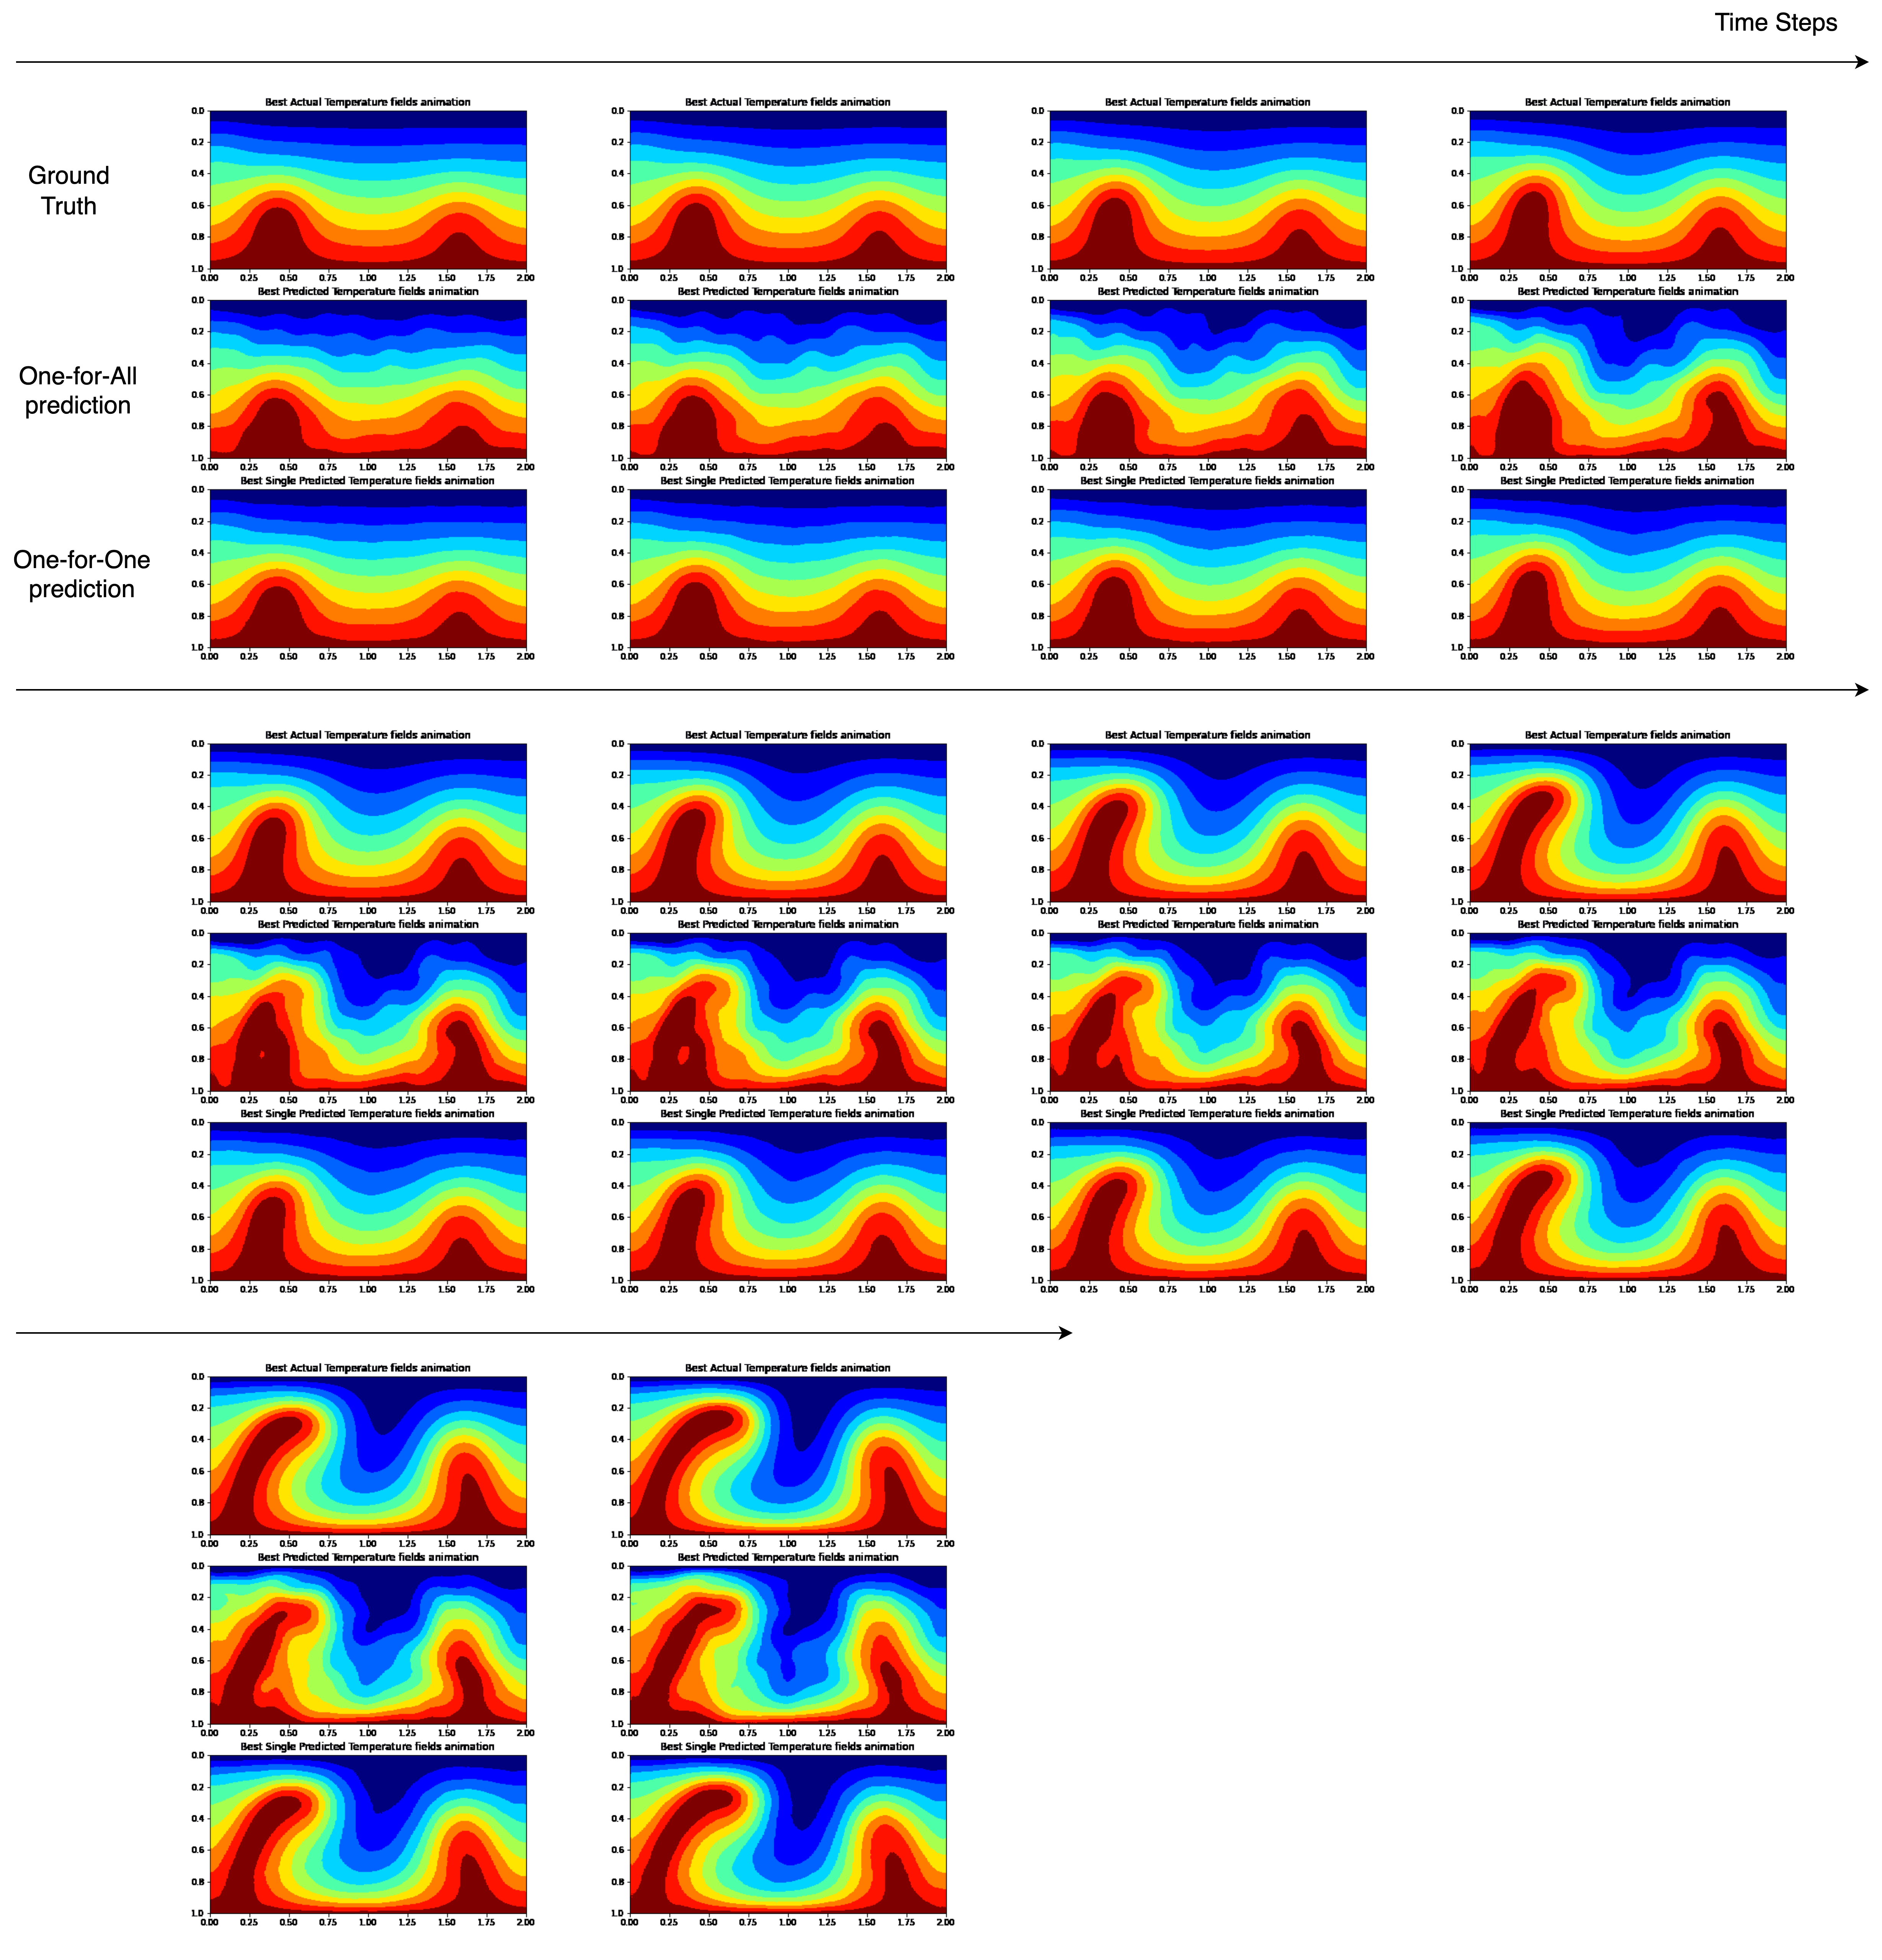
\includegraphics[width=\linewidth]{figures/FNN_animation_sheet.png}
    \caption{Best case animation sheet for FNN trained with Interpolated Dataset}
\end{figure}

\begin{itemize}
    \item Further Testings on FNN trained with Interpolated Dataset
        \begin{itemize}
            \item The aim is to determine experimentally for how many time steps we can use the trained FNN during a set of S consecutive time steps (e.g., S=2 and then ”correct” the time series with the truth coming from the simulator) without losing track of the transient dynamics (How large can S be without significantly affecting accuracy)

            \item The maximum value of S that is not significantly affecting accuracy should be 4 since the sum of loss and the sum of POD (Proper Orthogonal Decomposition) difference tend to have a rapid increase when S is increased from 4 to 8.
        \end{itemize}          
\end{itemize}

\begin{figure}[H]
    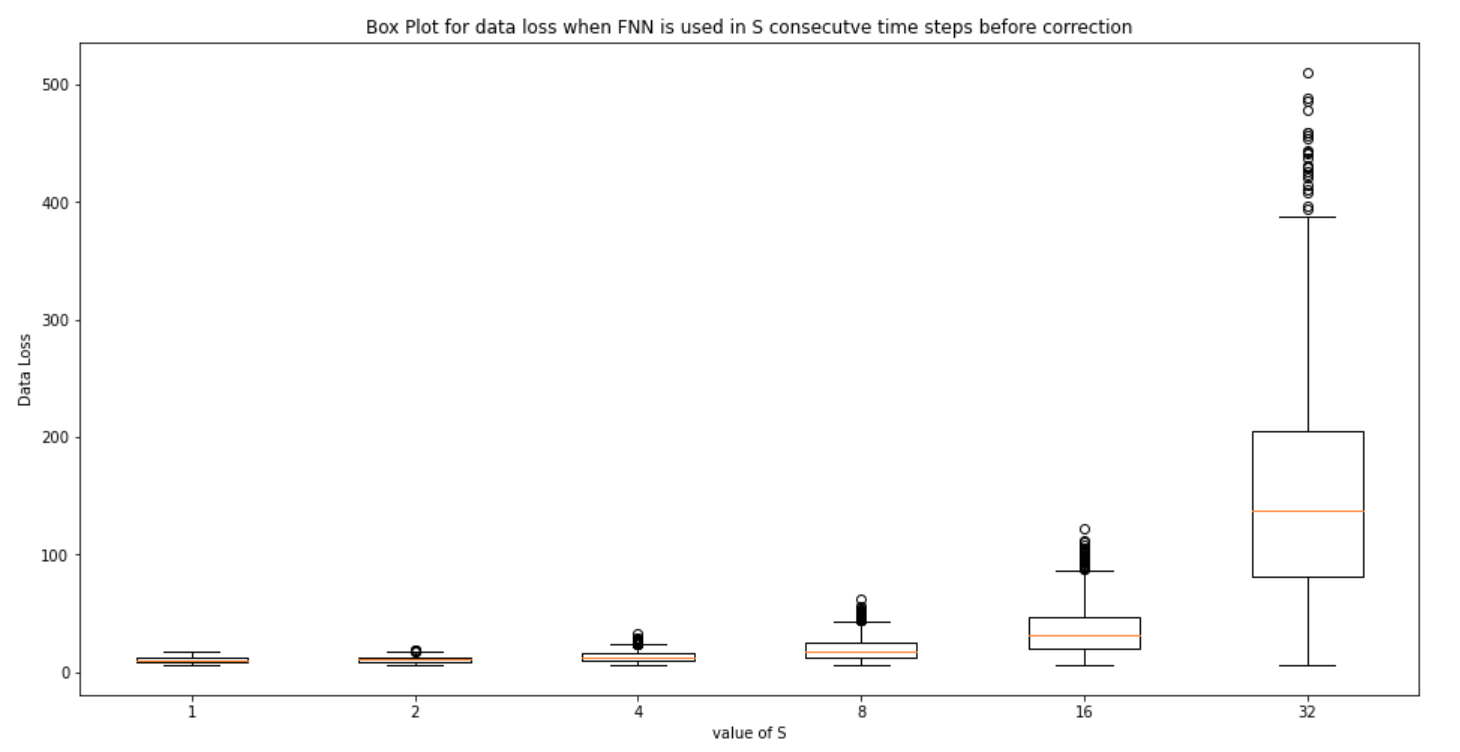
\includegraphics[width=\linewidth]{figures/FNN_boxplot.png}
    \caption{Box Plot for data loss when FNN is used in S consecutive time steps before correction}
\end{figure}

}

\Block{Results and Findings (Continue)}{
\begin{figure}[H]
    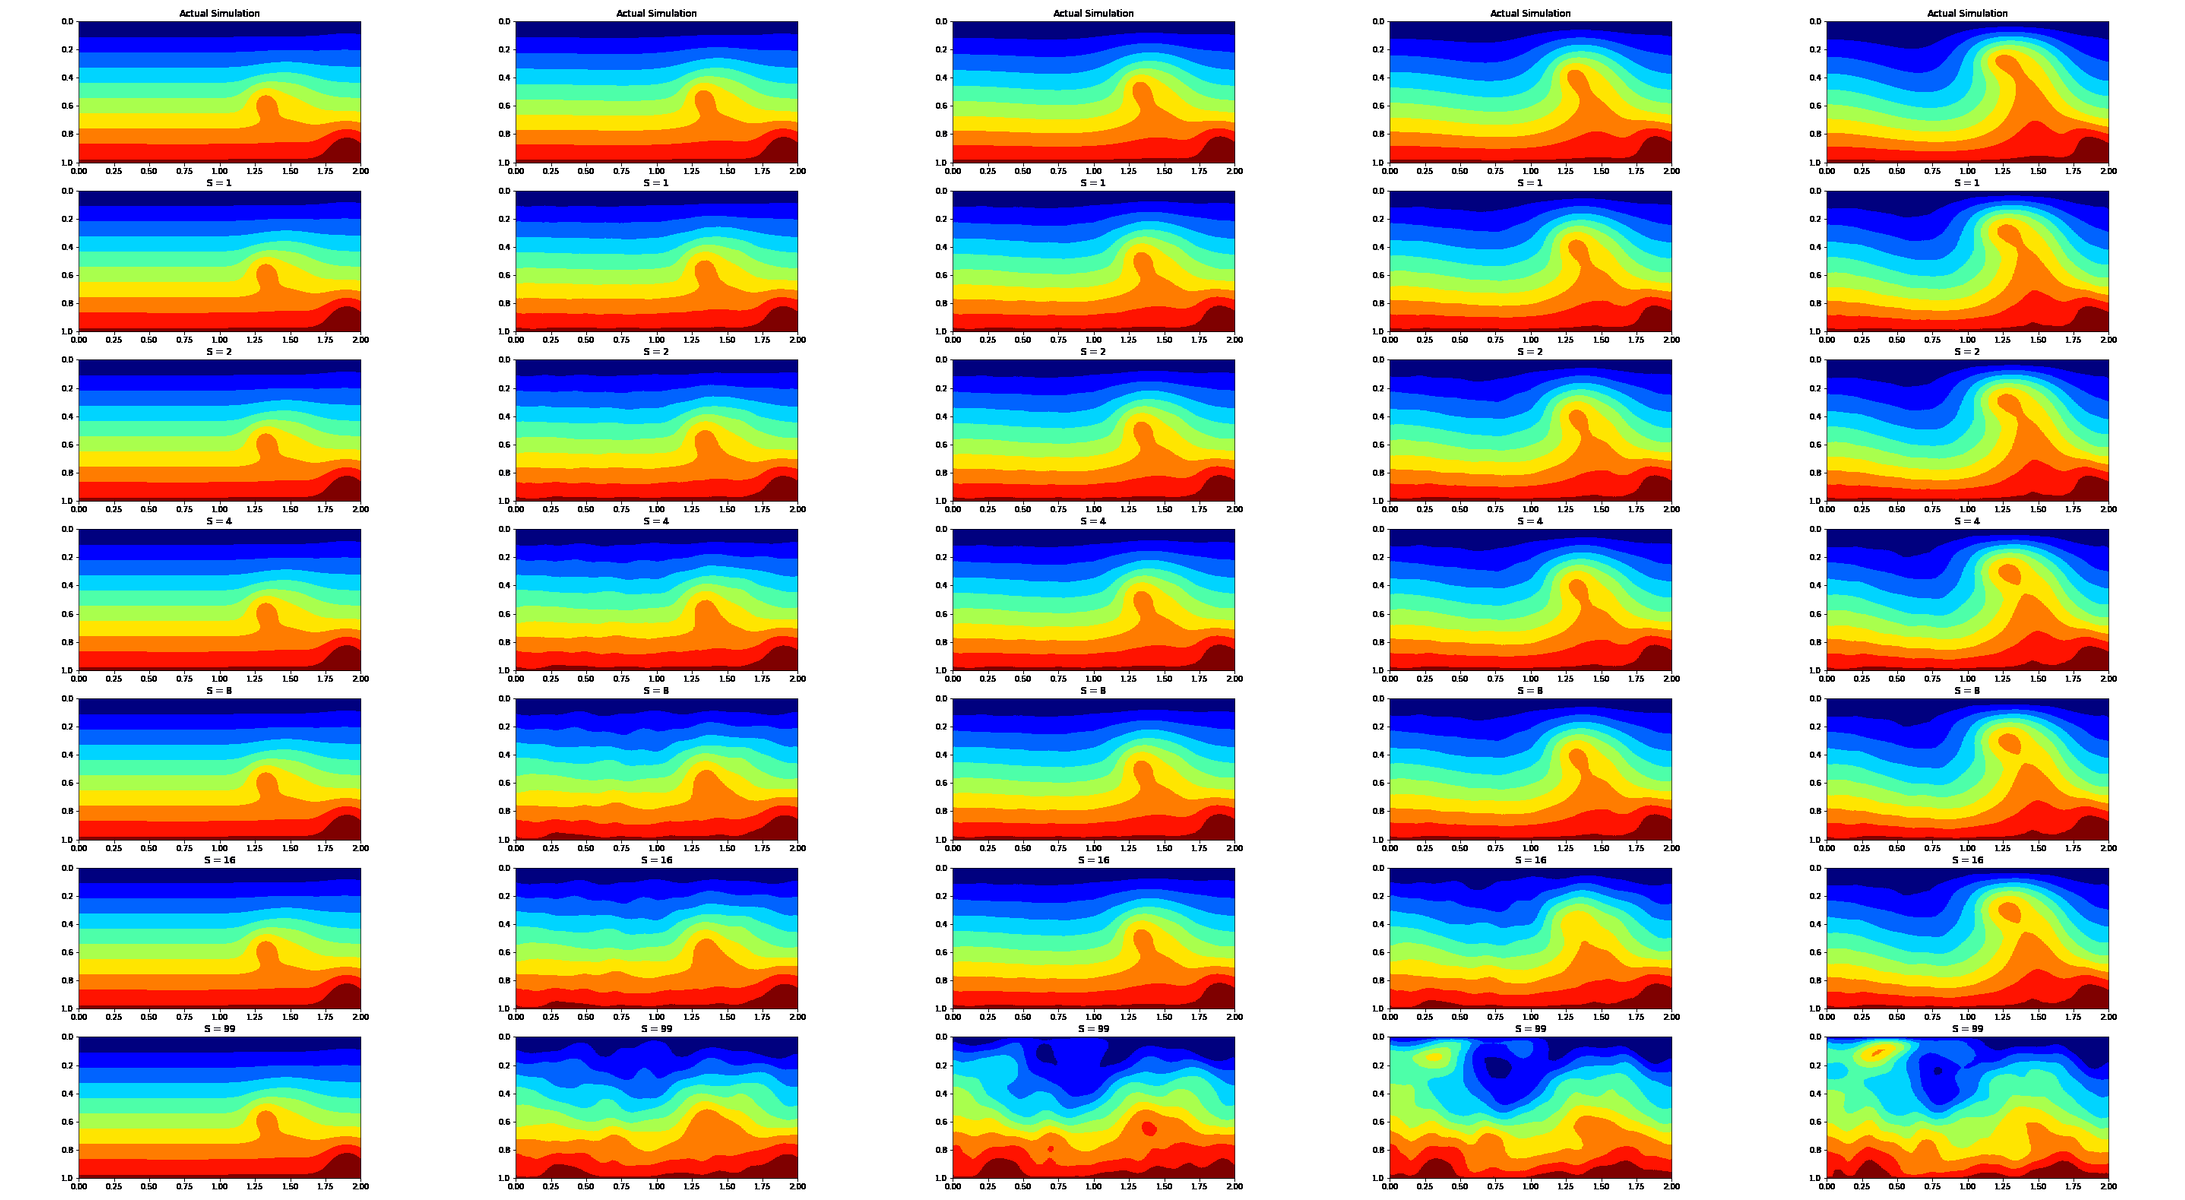
\includegraphics[width=\linewidth]{figures/FNN_further_testing_sheet.png}
    \caption{Animation sheet when FNN is either not used (ground truth at the first row) or used in S consecutive time steps before correction, where S = 1, 2, 4, 8, 16, 99 (started from the second row)}
\end{figure}
}

\Block{Conclusion}{
(TODO)
}


\Block{Future Works}{
\textbf{Mantle Convection Problem}

\begin{itemize}
     \item Future studies may continue to explore the potential use of the trained FNN on a set of S consecutive time steps. If we can somehow replace the fine-grained truth temperature field from the simulator (size is 201x401), that is used to "correct" the predicted time series, with a coarse-grained temperature field (e.g. size is 50x100), the computational complexity of modelling mantle convection problem could be further reduced.

     \item Future studies could also focus on improving the performance of LSTM or using less truth temperature fields to predict more temperature fields, rather than sticking to the current ratio of 50:50 for input and output due to the technical limitation of PyTorch.
\end{itemize}
}

\Block{Literature}{
\begin{itemize}
\item Agarwal, S.; Tosi, N.; Breuer, D.; Padovan, S.; Kessel, P.; and Montavon, G., 2020. A machine-learning-based surrogate model of mars’ thermal evolution.
Geophysical Journal International, 222, 3 (may 2020), 1656–1670. doi:10.1093/gji/ggaa234. https://doi.org/10.1093/gji/ggaa234.

\item Agarwal, S.; Tosi, N.; Kessel, P.; Breuer, D.; and Montavon, G., 2021. Deep learning for surrogate modeling of two-dimensional mantle convection. Physical
Review Fluids, 6, 11 (nov 2021). doi:10.1103/physrevf luids.6.113801. https://doi.org/10.1103/physrevfluids.6.113801.

\item Kerl, J., 2022. Geoid Inversion For Mantle Viscosity With Convolutional Neural Net-
works. Master thesis.
\end{itemize}
}